% Использован шаблон:
% https://www.writelatex.com/coursera/latex/1.1
% http://coursera.org/course/latex


\documentclass[a4paper,12pt]{article}

\usepackage{cmap}
\usepackage[T2A]{fontenc}
\usepackage[utf8]{inputenc}
\usepackage[english,russian]{babel}
\usepackage{fancyhdr}
\usepackage{minted}
\usepackage{hyperref}
\usepackage{amsmath}
\usepackage{graphicx}
\usepackage{xcolor}

\hypersetup{
  pdfborderstyle={/S/U/W 1}
}

\graphicspath{{./images/}}

\pagestyle{fancy}
\fancyhf{}
\lhead{Антон Завьялов, ПИ-72}
\rhead{\textbf{Лабораторная №2. Вариант 2}}
\cfoot{\thepage}

\makeatletter
\def\@seccntformat#1{%
  \expandafter\ifx\csname c@#1\endcsname\c@section\else
  \csname the#1\endcsname\quad
  \fi}
\makeatother

\begin{document} % Конец преамбулы, начало текста.

\begin{center}
  \textbf{Лабораторная работа №2 по дисциплине\linebreak"Компьютерная графика"\linebreak\linebreakВыполнил студент группы ПИ-72 Завьялов А.А.}\\
\end{center}

\section{\normalsize{Задание}}
\begin{flushleft}
  Сгенерировать 5-6 многоугольников (от 3 до 6 сторон) в пространстве и удалить невидимые части одним из методов.
\end{flushleft}

\begin{flushleft}
  \textbf{Вариант 2.} Простой алгоритм удаления невидимых ребер выпуклого тела с динамикой, например, вращение. Этот вариант допустимо выполнить на базе проволочного объекта из л.р. №1.
\end{flushleft}

\section{\normalsize{Ход работы}}
\begin{flushleft}
  \begin{enumerate}
    \item За основу взят код прошлой лабораторной работы.
    \item Модифицирован парсер файлов в формате \href{https://ru.wikipedia.org/wiki/Obj}{Wavefront OBJ}: помимо списка вершин и списка граней разбирается список нормалей, каждой грани соответствует свой вектор нормали.
    \item Реализован алгоритм выбраковки граней, экранируемых фигурой, основанный на исследовании взаимного положения нормали к плоскости и вектора, направленного от фигуры к наблюдателю.
    \item Алгоритм применен для тела в движении (случайный плавный поворот вокруг геометрического центра):
      \linebreak
      \begin{itemize}
        \item Для очередной грани, составляющей тело, координаты вектора нормали меняются согласно преобразованию.
        \item Выясняется взаимное положение вектора нормали и вектора к наблюдателю в мировых координатах.
        \item Если угол между векторами острый - грань видна наблюдателю, иначе - не видна.
        \item Тип угла между векторами можно легко определить при помощи скалярного произведения.
      \end{itemize}
    \item Для демонстрации работы алгоритма реализовано несколько надстроек:
      \linebreak
      \begin{itemize}
        \item Отображение координатных осей. Ось \textbf{OX} окрашена в {\color{red} красный} цвет, ось \textbf{OY} - в {\color{green} зеленый}, \textbf{OZ} - в {\color{blue} синий}. Включается/выключается нажатием на клавишу \textbf{a (ф)}.
        \item Отображение нормалей. Нормали к видимым граням окрашены в белый цвет, к невидимым граням окрашены в красный цвет. Включается/выключается нажатием на клавишу \textbf{n (т)}.
        \item Перевод из системы координат \((x,y,z)\) в \((y,x,z)\). В данном режиме можно наглядно увидеть взаимное положение вектора к наблюдателю (в системе \((x,y,z)\)) \((-p, 0, 0)\) и векторов нормалей. Включается/выключается нажатием на клавишу \textbf{r (к)}.
        \item Выключение/включение режима удаления невидимых граней на клавишу \textbf{z (я)}.
      \end{itemize}
  \end{enumerate}
\end{flushleft}

\section{\normalsize{Исходный код}}
Исходный код программы также расположен в Git-репозитории по адресу: \url{https://github.com/andiogenes/cg/tree/master/backface-culling}
\inputminted[breaklines]{python}{../culling.py}

\section{\normalsize{Демонстрация работы программы}}
\begin{flushleft}
  Полигональное тело из прошлой лабораторной работы (\textit{обезьяна Сьюзен} из пакета 3D-моделирования \textbf{Blender}) не является выпуклым, поэтому для данной лабораторной работы был подготовлен новый набор трехмерных примитивов:
\end{flushleft}
\begin{flushleft}
  Тетраэдр:\linebreak
  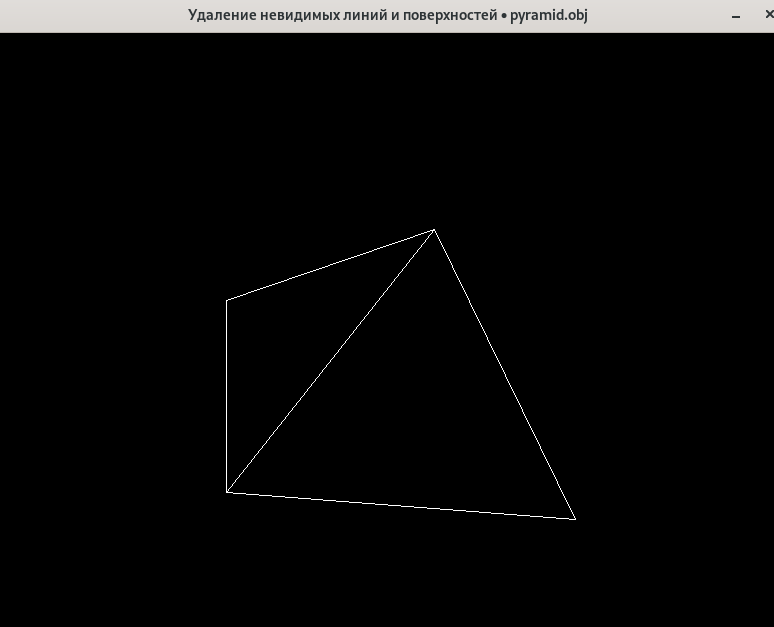
\includegraphics[scale=1.5]{pyramid.png}\linebreak\linebreak
  Куб:\linebreak
  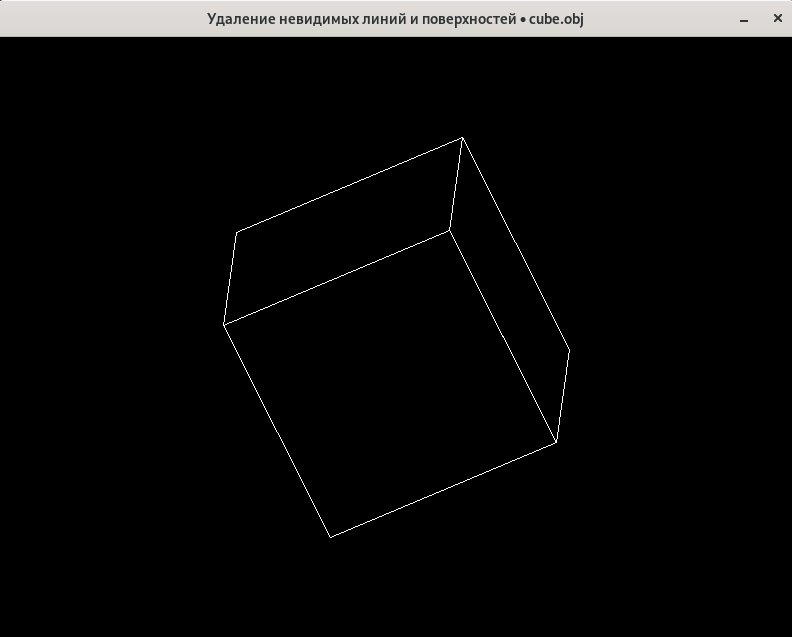
\includegraphics[scale=1.5]{cube.png}\linebreak\linebreak
  Цилиндр:\linebreak
  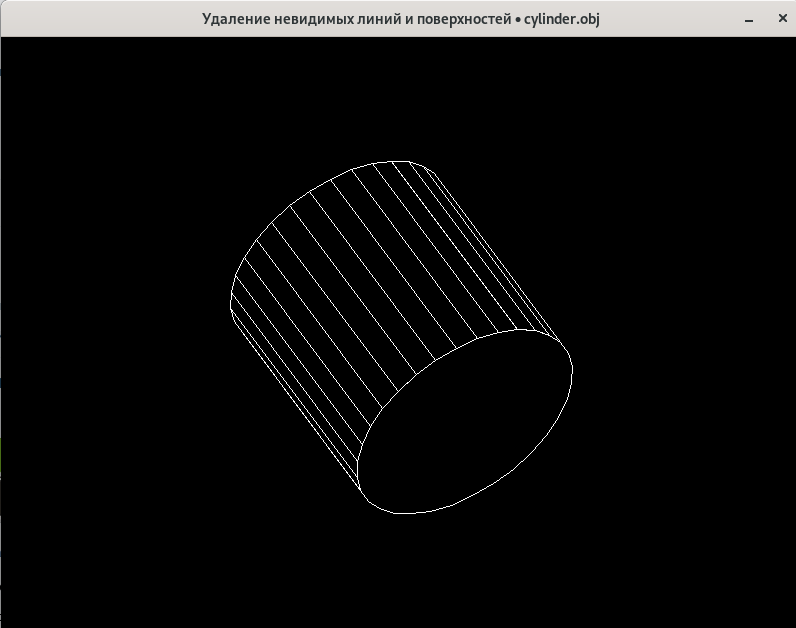
\includegraphics[scale=1.5]{cylinder.png}\linebreak\linebreak
  Икосаэдр:\linebreak
  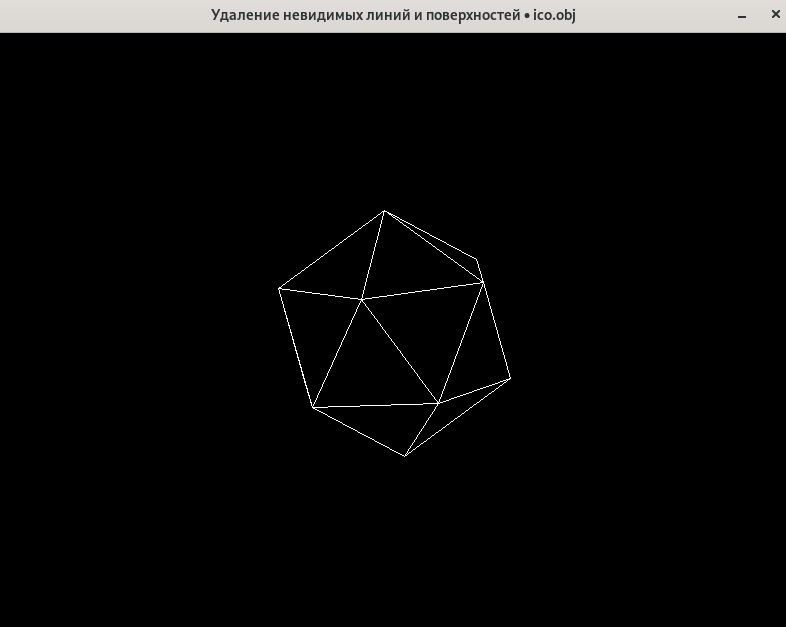
\includegraphics[scale=1.5]{ico.png}\linebreak\linebreak
  Сфера:\linebreak
  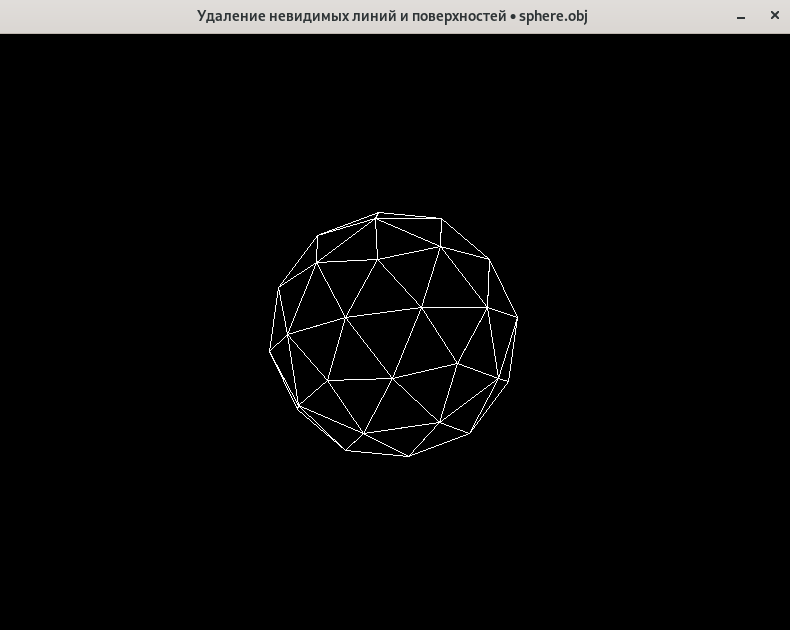
\includegraphics[scale=1.5]{sphere.png}\linebreak\linebreak
  Отображение нормалей:\linebreak
  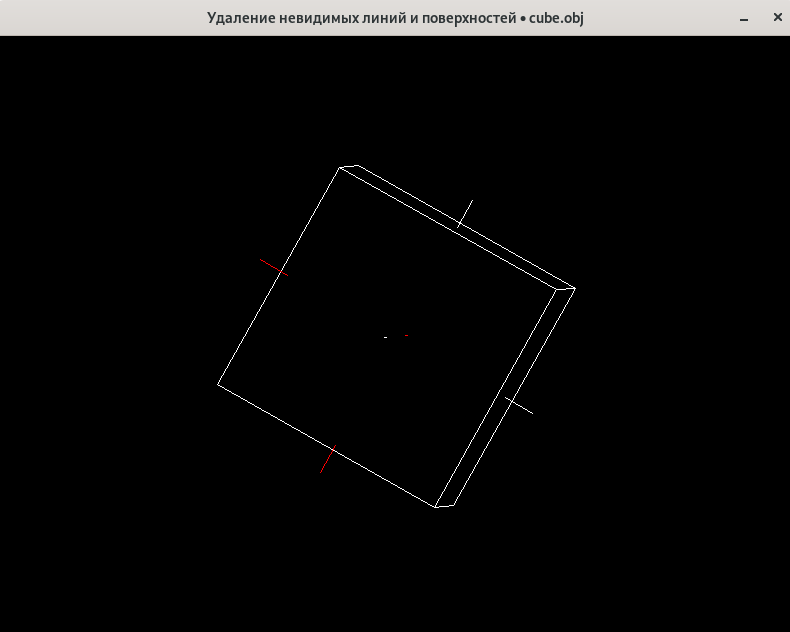
\includegraphics[scale=1.5]{normals_cube.png}\linebreak\linebreak
  "Вид сбоку":\linebreak
  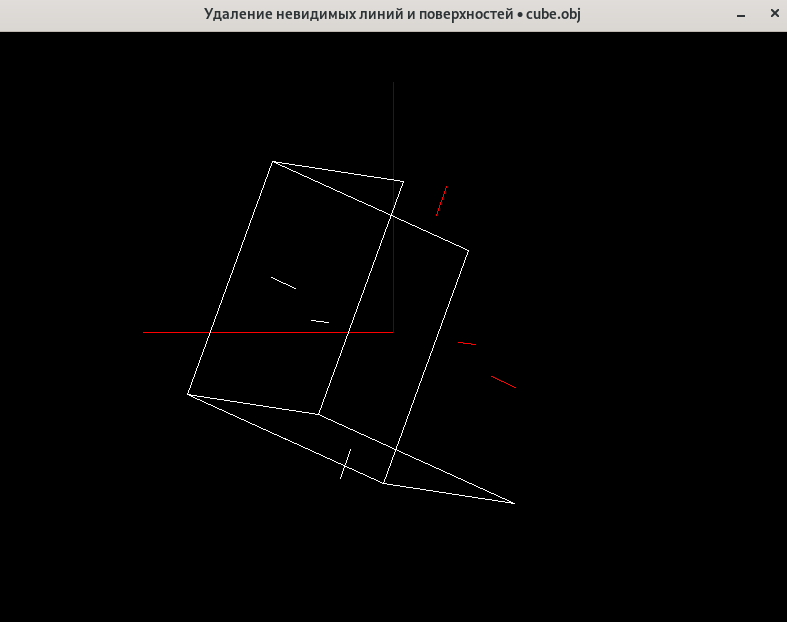
\includegraphics[scale=1.5]{axis_rotate_normals.png}\linebreak
  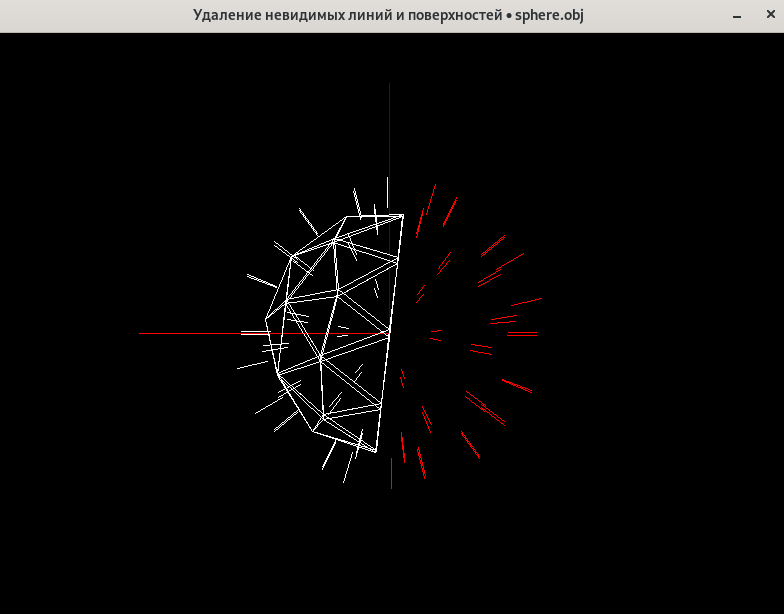
\includegraphics[scale=1.5]{sphere_rotate_normals.png}
\end{flushleft}
\begin{flushleft}
  \textbf{Демонстрацию анимации можно посмотреть на YouTube:} \url{https://youtu.be/fUeFCBrGxwQ}
\end{flushleft}
\end{document}

